\chapter{Realizacja biometrycznego systemu kontroli dostępu}
\label{cha:realizacja}
~W tym rozdziale przedstawiono sposób realizacji biometrycznego systemu do kontroli dostępu, ~wykorzystującego obraz tęczówki oka jako elementu na podstawie którego następuje rozpoznanie. System ten składa się ze stanowiska służącego do akwizycji obrazu oka, algorytmów przetwarzających pobrany obraz, generujących ~i porównujących kody tęczówek oraz aplikacji, mającej na celu ułatwienie korzystania ~z funkcji systemu ~i zapewniającej dostęp do bazy danych przechowującej informacje. Jest on rozbudowaną ~wersją systemu opracowanego ~w pracy \cite{Gl11}, opartą ~o zaprezentowaną ~w niej aplikację. W niniejszej pracy do poprzedniego systemu ~wprowadzony został szereg ulepszeń, zarówno pod kątem poprawy algorytmu działania, jak ~i ~wzbogacenia interfejsu użytkownika oraz bazy danych, służącej do przechowywania informacji dotyczących rozpoznawanych osób.
%~W tym rozdziale przedstawiono sposób realizacji systemu do kontroli dostępu ~wykorzystującego obraz tęczówki oka jako elementu na podstawie, którego następuje rozpoznanie. System składa się ze stanowiska do akwizycji obrazu tęczówki oka oraz aplikacji generującej kod tęczówki oraz porównującej kody ze sobą. Aplikacja składa się ~z kliku modułów: ~wykrycie źrenicy, ~wykrycie granic tęczówki, tworzenie kodu tęczówki oraz ewentualnie porównania ~wygenerowane kodu ~z już istniejącym.

\section{Stanowisko do akwizycji obrazu oka}
\label{sec:stanowisko}
Skonstruowane na potrzeby pracy stanowisko do akwizycji obrazu oka zostało oparte na pierwowzorze przedstawionym ~w pracy \cite{Gl11}. Rekonstrukcja nastąpiła ~w dwóch etapach. W pierwszym zastosowano kamerę ~o odmiennych od opisanych ~w pracy \cite{Gl11} parametrach, jednakże ~w związku ~z niewystarczającą jakością pobranych ~z jej pomocą obrazów, postanowiono podjąć kolejną próbę konstrukcji stanowiska, ~z użyciem poprzedniej kamery oraz obiektywu ~o lepszych parametrach.

Stanowisko złożone zostało ~z następujących elementów:
\begin{itemize}
 \item kamery cyfrowej, mającej za zadanie pobieranie obrazu ~w formie filmu bądź pojedynczych zdjęć,
 \item obiektywu ~o odpowiedniej ostrości ~i innych kluczowych parametrach,
 \item statywu, służącego do podtrzymywania ~i stabilizacji kamery,
 \item specjalnego stojaka, umożliwiającego poprawne ~i ~wygodne ułożenie głowy osoby, która jest identyfikowana,
 \item kartonowego pudła, ~w którym umieszczone zostały kamera ~i obiektyw oraz do którego częściowo ~wsunięty został stojak,
 \item lampy, generującej oświetlenie ~w celu uzyskania jak najwęższego rozmiaru źrenicy oka ~z przytwierdzonym fragmentem tworzywa pleksi rozpraszającego promienie światła.
 \end{itemize}

Podczas pierwszej próby konstrukcji stanowiska, jako urządzenie pobierające obraz oka ~wybrano kamerę firmy , ~o następujących parametrach:

Wybór urządzenia był ograniczony zasobami laboratorium, ~w którym było tworzone stanowisko. Kamera została umieszczona na statywie, ~w celu regulacji jej położenia ~i stabilizacji pobieranego obrazu.

Do ~wybranej kamery należało dobrać obiektyw. Ponieważ podstawowym celem akwizycji było otrzymanie ostrego obrazu ~o dużym powiększeniu oraz odpowiedniej głębi ostrości, należało ~wybrać obiektyw ~o możliwie dużej ogniskowej. Zdecydowano się ~wykorzystać najlepszy dostępny ~w laboratorium obiektyw, !!!!!TU WSTAWIĆ NAZWĘ!!!!.

Po odpowiednim ustawieniu opisanych urządzeń, na ~wprost kamery umieszczono stojak, mający na celu podtrzymanie głowy osoby identyfikowanej. Został on ustawiony na ~wysokości odpowiadającej położeniu komfortowemu dla ~większości osób, ~z umożliwieniem jego ewentualnej modyfikacji.

Następnie podjęto próby akwizycji obrazu. Po zapisaniu zdjęć pobranych przy pomocy kamery, istotnym problemem okazały się być odblaski, powstałe na powierzchni oka ~w ~wyniku odbicia światła zewnętrznego, pochodzącego ~z otoczenia lub sztucznych źródeł, takich, jak żarówki. Odblaskami stanowiącymi największą przeszkodę były obecne na tęczówce oraz źrenicy, ponieważ te elementy obrazu są kluczowe dla dalszej analizy. Najprostszym sposobem eliminacji tego rodzaju zakłóceń jest ograniczenie dostępu promieni świetlnych ~z otoczenia do obszaru, ~w którym pobierany jest obraz. Udało się to zrealizować, podobnie jak ~w \cite{Gl11}, za pomocą umieszczenia kamery ~w kartonowym pudełku, na granicy którego ustawiono stojak stabilizujący głowę. Metoda ta pozwoliła na ograniczenie odblasków do minimum oraz uzyskanie odpowiedniej ostrości obrazu poprzez unieruchomienie głowy osoby identyfikowanej.

Wadą zastosowanego rozwiązania było jednak zmniejszenie jasności uzyskiwanych obrazów. Przyczyniło się to do rozszerzenia źrenicy oka, co miało negatywny ~wpływ na długość promienia tęczówki. W celu rozjaśnienia obrazu użyto ~więc oświetlacza IR oraz lampy umieszczonej na kamerze, której zadaniem było oświetlenie oka badanej osoby ~i ~w konsekwencji zwężenie obszaru źrenicy. Takiego rodzaju oświetlenie również tworzy odblaski, lecz ~w tym ~wypadku mogą być one ~wykorzystane przez algorytm ~wykrywający źrenicę. Jest to możliwe, ponieważ ~z uwagi na umiejscowienie lampy odblask powstaje na środku źrenicy, dzięki czemu ułatwiona zostaje jej lokalizacja. (Dodać coś ~o oświetlaczu IR). Obraz jest zapisywany ~w skali szarości.

Pobierany obraz zapisywany był ~w skali szarości ~i formacie BMP, co umożliwiło łatwiejsze jego przetwarzanie przez algorytm. Po ~wykonaniu odpowiedniej ilości testów programu na pobranych zdjęciach, okazało się jednak, iż nie cechowały się one ~wystarczająco ~wysoką jakością, która konieczna była dla poprawnego działania algorytmów generujących ~i porównujących kody tęczówek. W związku ~z tym, niezbędna była ponowna rekonstrukcja stanowiska, tym razem ~z zastosowaniem kamery ~o sprawdzonej skuteczności pobierania obrazu, użytej ~w pracy \cite{Gl11}.

W trakcie drugiej próby konstrukcji stanowiska, zdecydowano się na zastosowanie urządzenia firmy ~o parametrach: . Problemem ~wywołującym trudności podczas pobierania obrazów przy pomocy poprzedniej kamery była jej mała rozdzielczość, co udało się pokonać stosując nową kamerę. Ponadto, ~wewnątrz kartonowego pudełka jasność otoczenia była zbyt niska, pomimo użytej lampy, jednak udało się to zniwelować ~wyłącznie ~z użyciem oświetlacza IR, dzięki czemu na obrazie ~widocznych było mniej odblasków. Oświetlacz został zamontowany na kamerze.

Postanowiono pozostać przy obiektywie, który został użyty podczas pierwszej konstrukcji stanowiska. Pozostałe części, takie, jak kartonowe pudełko, stojak, statyw oraz oświetlacz IR również nie uległy modyfikacji.

\section{Część biometryczna - ~wykrywanie tęczówki oka na obrazie ~i identyfikacja bądź ~weryfikacja tożsamości na jej podstawie}
\subsection{Wykrywanie źrenicy na pobranym obrazie}
\label{sec:wykrycieZrenicy}

Część algorytmu odpowiedzialna za ~wykrycie źrenicy ma za zadanie odnalezienie tej części oka ludzkiego na obrazie oraz opisanie jej kształtu ~w formie okręgu ~o odpowiednich parametrach. Zadanie to jest realizowane ~z ~wykorzystaniem opisanego ~w podrozdziale \ref{sec:stanowisko} odblasku, pochodzącego od lampy ustawionej na kamerze, Powinien on znajdować się ~w centrum źrenicy, dlatego też konieczne jest ustawienie ~we ~właściwej pozycji osoby, której zdjęcie jest pobierane przez kamerę. Odblask jest jednym ~z najjaśniejszych punktów na obrazie. ~W związku ~z tym, ~wykrycie odblasku odbywa się poprzez ~wykorzystanie binaryzacji ~z progiem 254. W ~wyniku tej operacji na obrazie zostają tylko piksele najjaśniejsze (jak na rysunku \ref{fig:binaryzacja}). Niestety na ~wielu ujęciach odblask na źrenicy nie jest jedynym, który jest ~widoczny na obrazie. Pozostałe mogą znajdować się ~w różnych miejscach: na białku oka lub na skórze. Można ten fakt ~wykorzystać poprzez analizę otoczenia znalezionych odblasków. 

\begin{figure}
\begin{center}
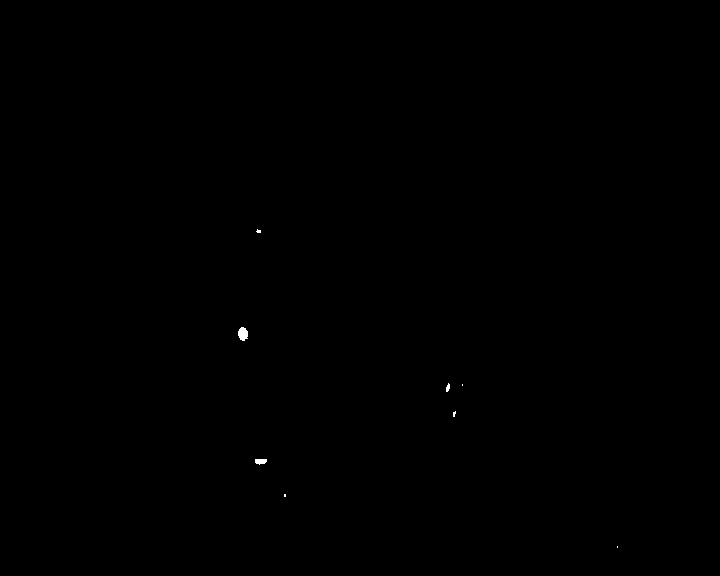
\includegraphics[scale=0.5]{binaryzacja.jpg}
\caption{Obraz po binaryzacji, jasne punkty to znalezione odblaski}
\label{fig:binaryzacja}
\end{center}
\end{figure}

Najistotniejszy dla dalszych etapów algorytmu odblask znajduje się ~w otoczeniu źrenicy, ~a ~więc jednego ~z najciemniejszych obszarów obrazu; otoczenie pozostałych odblasków jest ~o ~wiele jaśniejsze (skóra lub białko oka). ~W obrazie uzyskanym po binaryzacji wyszukiwane są piksele odblasku. ~W momencie znalezienia każdego kolejnego piksela odblasku analizowane jest jego otoczenie. Sprawdzanych jest po 10 punków na ukos ~w górę ~z lewej ~i prawej strony. Jeśli większość z nich ma jasność poniżej 60 to analizowany piksel jest uznawany za piksel odblasku znajdującego się na źrenicy. W takiej sytuacji wyszukiwanie zostaje zakończone i następuje dalsza cześć algorytmu.

Następnie wyszukiwany jest cały odblask. Odbywa się to poprzez analizę otoczenia (kwadratu o boku 50 pikseli oraz środku w miejscu już znalezionego fragmentu) znalezionego punktu. Sprawdzany jest każdy piksel ~w wybranym otoczeniu i uznawany jest za element odblasku w sytuacji, gdy jego jasność jest większa niż 240. Przykład wyniku przeprowadzonych operacji jest przedstawiony na rysunku \ref{fig:dobryOdblask}.

\begin{figure}
\begin{center}
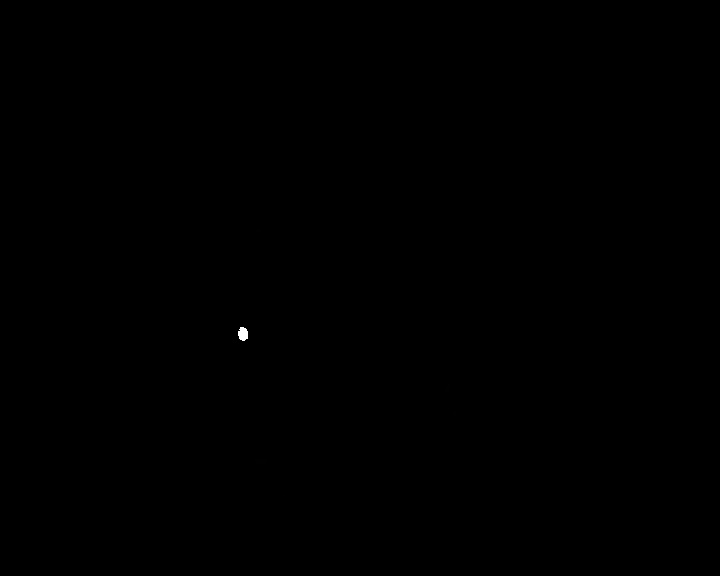
\includegraphics[scale=0.5]{odblask.jpg}
\caption{Obraz po realizacji algorytmu poszukiwania odblasku na źrenicy}
\label{fig:dobryOdblask}
\end{center}
\end{figure}

Po znalezieniu ~wszystkich pikseli należących do odblasku, jego kształt jest aproksymowany przy pomocy koła, którego środek jest przyjmowany jako środek źrenicy. Mając środek źrenicy można zastosować metodę ,,eksplodujących okręgów'', zaczerpniętych ~z patentu Daugmana.  Szukany jest największy wzrost jasności pikseli na rozszerzającym się okręgu (~z uwagi na to, że źrenica jest ciemna, ~a tęczówka jest jaśniejsza). Znaleziony okrąg określa źrenicę. Niestety dla zarejestrowanych obrazów metoda nie okazała się skuteczna. Z tego powodu zastosowano nieco odmienną metodę. Wyszukiwanie odbywa się na promieniach, to znaczy wybierane są 72 promienie ~o różnych kierunkach ~i na każdym wyszukiwany jest największy wzrost jasności. Dla znalezionych punktów wyszukuje się najmniejszy okrąg, ~w którym zawierają się wszystkie punkty. Stosowany jest algorytm zaimplementowany w bibliotece OpenCV. Znaleziony okrąg określa źrenicę. Przykład obrazu ~z ~wykrytą źrenicą jest przedstawiony na rysunku \ref{fig:zrenicaNasza}.

\begin{figure}
\begin{center}
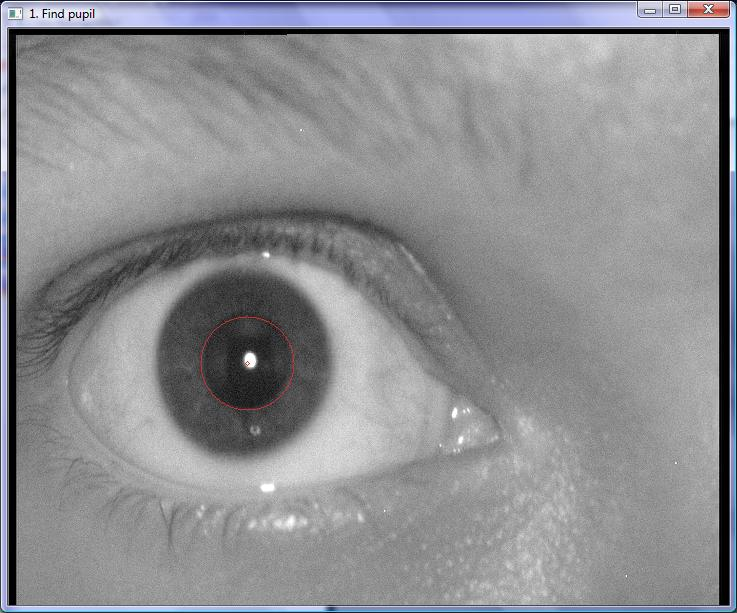
\includegraphics[scale=0.5]{zrenica.jpg}
\caption{Wykryta źrenica}
\label{fig:zrenicaNasza}
\end{center}
\end{figure}

Po zmianie kamery algorytm ~wykrywania źrenicy został zmieniony. Było to spowodowane poprawą jasności zdjęcia oraz zmianą położenia niektórych elementów stanowiska. Odblask na źrenicy, ~wcześniej będący się ~w środku źrenicy po zmienie stanowiska znajduje się ponad środkiem. W związku ~z tym nie można go ~wykorzystać do ustalenia środka źrenicy.

Można natomiast ~wykarzystać ~wykrycie odblasku do oszacowania, ~w którym miejscu na obrazie znajduje się źrenica. Pozwala to ograniczyć ~wielkość obrazu podlegającemu późniejszym przekształceniom. Wybierany jest kwadrat ~o boku 440 pikseli. Taki obszar jest ~wystarczający, ponieważ promień źrenicy na rejestrowanych obrazach nie przekracza 150 piksleli. Taki zabieg pozwala na osiągnięcie dwóch korzyści. Pierwszą jest zmniejszenie obszaru, który podlega przekształceniom co przyśpiesza działanie programi. Drugą jest ograniczenie innych obiektów na zdjęciu, jak brwi czy rzęsy, które mogą być uznane podczas binaryzacji za fragmenty źrenicy. Pozwala to na ograniczenie błędów podczas segmentacji. W tym obszarze przeprowadzna są następujące operacje:
\begin{itemize}
\item Najpierw stosowana jest binaryzacja ~z dwoma programi, ~wybierane są piksele należące do źrenicy (o jasności mniejszej niż 60) oraz piksele należące do odblasku (o jasności 255). Dzięki temu, otrzymuje bardziej zwarty obszar źrenicy. Po tej operacji powstaje obraz \ref{fig:binaryzacja2}, na którym ~widać ~większą część źrenicy.
\begin{figure}
\begin{center}
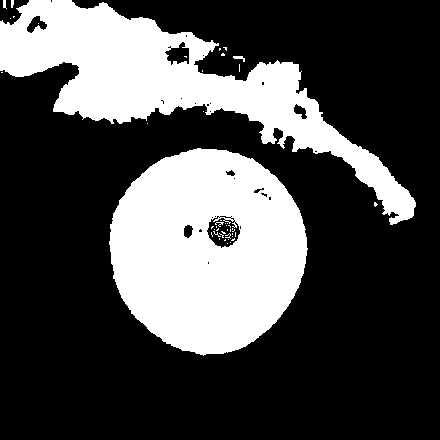
\includegraphics[scale=0.5]{binaryzacja2.jpg}
\caption{Wykryta źrenica}
\label{fig:binaryzacja2}
\end{center}
\end{figure}
\item Zamknięcie, po którym obszary znajdujące się ~w środku źrenicy ~w otoczeniu odblasku, które mają mniejszą jasność niż on sam zostają ~włączone do obszaru źrenicy. Na obrazie \ref{fig:zamkniecie2} po tej operacji ~wyraźnie ~widać, że źrenica jest ~wyznaczona ~w całości.
\begin{figure}
\begin{center}

\includegraphics[scale=0.5]{zamkniecie.jpg}
\caption{Wykryta źrenica}
\label{fig:zamkniecie2}
\end{center}
\end{figure}
\item Dwuktrotne otwarcie, po którym usuwane są ~w ~większej części obszary rzęs, które pozostają po ~wcześniejszych operacjach. Czasem po binaryzacji powstaje obraz, na którym rzęsy są połączone ze źrenicą. Ta operacja pozwala rozdzielić je od siebie.
\begin{figure}
\begin{center}
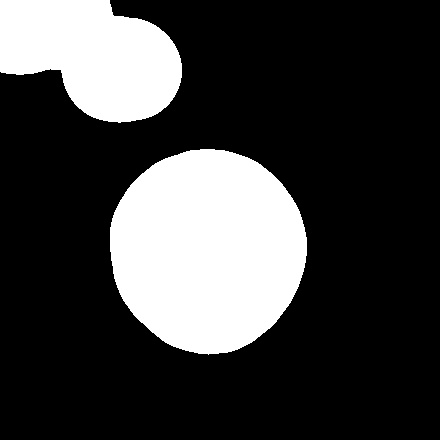
\includegraphics[scale=0.5]{otwarcie2.jpg}
\caption{Wykryta źrenica}
\label{fig:otwarcie2}
\end{center}
\end{figure}
\item Czyszczenie brzegów ~w ramach ~wybranego ~wcześniej obszaru. Po tej operacji na obrazie zostaje sama źrenica ~i znikają ewentualne pozostałości po ~wykrytych rzęsach. Jest to ostatni etap ~wyznaczania obszaru źrenicy ~i otrzymujemy obraz \ref{fig:zrenica2}.
\begin{figure}
\begin{center}
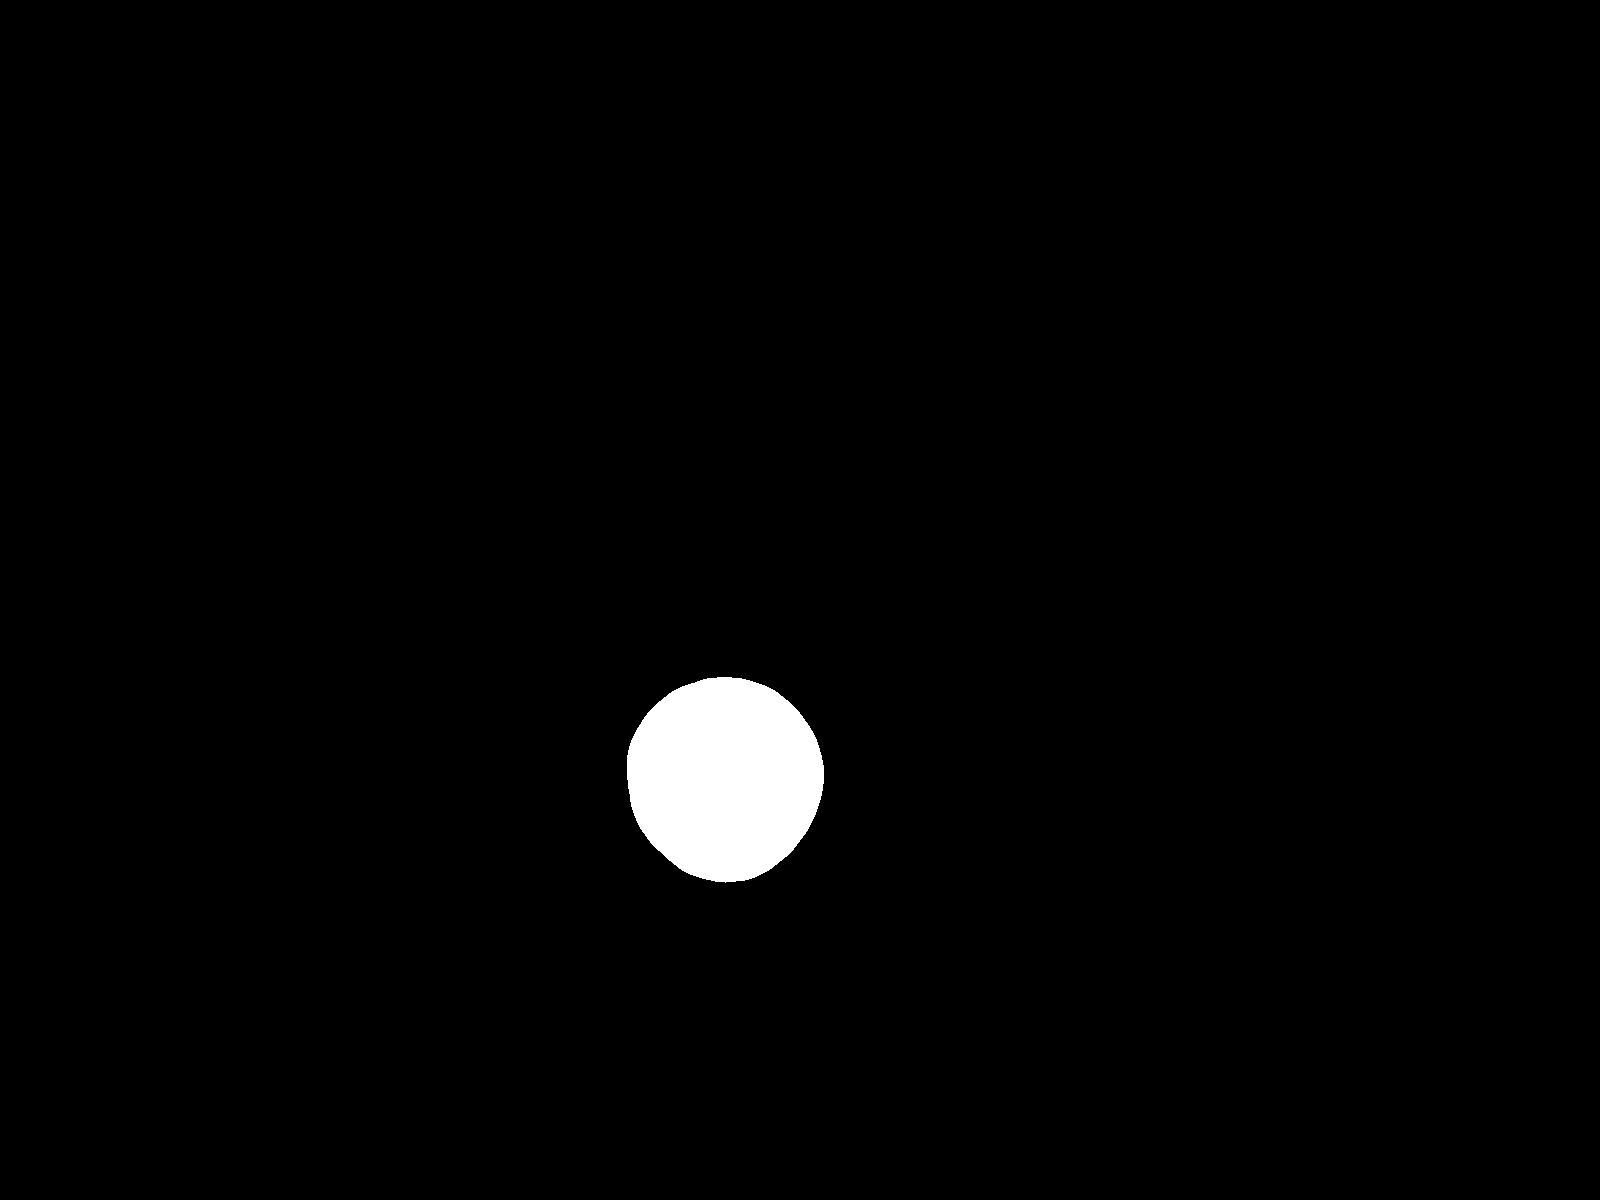
\includegraphics[scale=0.5]{zrenica2.jpg}
\caption{Wykryta źrenica}
\label{fig:zrenica2}
\end{center}
\end{figure}
\end{itemize}


\section{Wykrycie tęczówki}
\label{sec:wykrycieTeczowki}
Algorytm odpowiedzialny za ~wykrycie tęczówki oparty został na użytym ~w pracy \cite{Gl11}. Przykładowy obraz ~z ~wykrytą tęczówką jest przedstawiony na rysunku \ref{fig:teczowkaNasza}.
\begin{figure}
\begin{center}
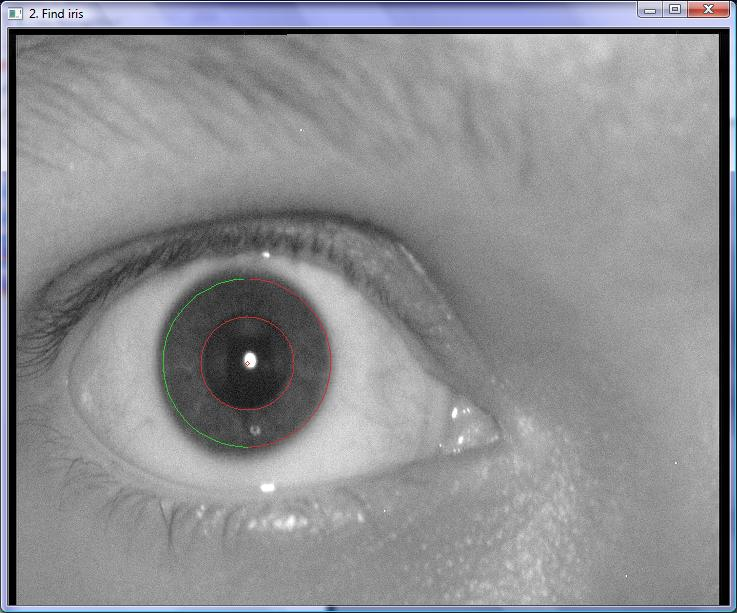
\includegraphics[scale=0.5]{teczowka.jpg}
\caption{Obraz po realizacji algorytmu poszukiwania granic tęczówki}
\label{fig:teczowkaNasza}
\end{center}
\end{figure}

\section{Ekstrakcja cech tęczówki}
\label{sec:ekstrakcja}
Zadaniem części algorytmu odpowiedzialnej za ektrakcję cech tęczówki jest ograniczenie ilości danych reprezentujących daną tęczówkę. Po przeprowadzeniu tej operacji zostaje utworzony ~wektor ~o długości 2048 bitów. Dzięki temu można znacznie zmniejszyć rozmiar przechowywanych danych, potrzebnych do poprawnego rozpoznania osoby. Ważne jest, by otrzymany ~wektor był ~wyraźnie odmienny dla różnych osób oraz aby dla jednej osoby różne zdjęcia generowały podobny zestaw bitów. 

~w celu określenia cech danej tęczówki stosuje się filtry Gabora określone ~wzorem (tu będą ~wzory ale na linuxie to zrobię)

Obraz jest przetwarzany ~z użyciem ~wspomnianych filtrów. Po tym zabiegu otrzymujemy ~współczynniki zespolone, które sumujemy ~w pewnych obszarach. Obszary ~wybierane są na powierzchni tęczówki ~w punktach zależnych od jej rozmiaru. Jest to spowodowane tym, że ~w zależności od jasności otoczenia źrenica zwiększa się lub zmniejsza, co powoduje zwężenie lub rozszerzenie tęczówki. Otrzymane sumy kodowane są ~w ten sposób, że osobno rozpatrując część rzeczywistą ~i urojoną, zapisywane jest 1 ~w przypadku, gdy suma jest ~większa od zera oraz 0 jeśli jest mniejsza lub równa. ~w ten sposób otrzymujemy 2 bity na jeden obszar. Ponieważ stosowane jest 8 różnych orientacji filtru Gabora, potrzebny jest ~wybór 2048/(2*8) = 128 obszarów. Obszary ~wybierane są po dwóch stronach tęczówki, ~więc ~wymagany jest ~wybór 64 obszarów na każdej stronie. Przykład ~wyznaczonych obszarów przedstawiony jest na rysunku \ref{fig:obszaryNasze}.

\begin{figure}
\begin{center}
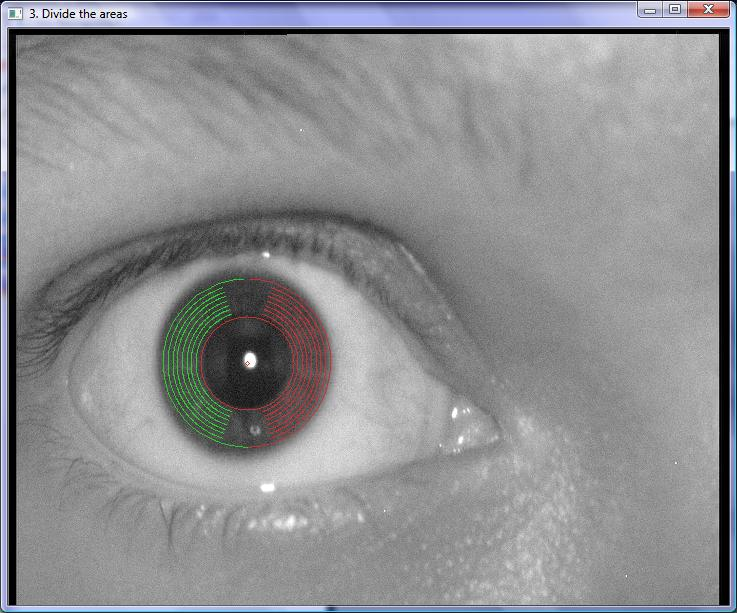
\includegraphics[scale=0.5]{obszary.jpg}
\caption{Obraz ~z zaznaczonymi obszarami używanymi do tworzenia kodu tęczówki}
\label{fig:obszaryNasze}
\end{center}
\end{figure}

\subsection{Porównanie kodów tęczówki}
\label{subsec:porownanieKodow}
~W celu określenia, czy dane dwie tęczówki należą do tej samej osoby, niezbędne jest porównanie otrzymanych kodów. Porównanie ~wykonywane jest za pomocą operacji XOR zgodnie ze ~wzorem \ref{eq:Hamming}.
\begin{equation}
\label{eq:Hamming}
H = \frac{\sum XOR(A,B)}{2048}
\end{equation}
gdzie:
$A, B$ - porównywane kody tęczówek, każdy ~o długości 2048 bitów.\\
Po tej operacji ~wartość $H$ określa procent różnych pikseli dla dwóch różnych kodów.

Głowa danej osoby może być ~w pozycji nieznacznie obróconej ~w trakcie pobierania zdjęcia służącego identyfikacji ~w stosunku do zdjęcia, ~na podstawie  którego powstał kod zapisany  ~w bazie. ~W celu zminimalizowania błędu stosowana jest rotacja jednego ~z porównywanych kodów. Kod jest przesuwany ~w obydwie strony ~o dwa piksele (ponieważ ~z jednej lokalizacji na obrazie otrzymujemy dwa bity kodu). Wykonywanych jest 9 porównań kodów. Wybierana jest najniższa ~wyliczona ~wartość odległości Hamminga. Ustalonym progiem zgodności dwóch kodów jest 0.18 \cite{Daugman}.

